\documentclass[a4paper,11pt,french]{article}

\usepackage[TD]{../../../Style}

%\renewenvironment{center}{\par \centering }{ \par}
%\renewenvironment{multicols*}[1]{}{}
%\setstretch{1.2}
\renewcommand{\arraystretch}{1.8}
% Début du document
%%%%%%%%%%%%%%%%%%%
\begin{document}

\titre{Probabilités}

\begin{multicols*}{2}

\section{Loi de probabilité}

\begin{exercice}
Une urne contient cinq boules numérotées de 1 à 5. On tire une boule au hasard et on lit le numéro obtenu. La probabilité de tomber sur chaque boule est reportée dans le tableau ci-dessous:

\begin{center}
\begin{small}
\begin{tabularx}{0.9\linewidth}{|c|*{5}{Y|}} \hline
Issue & 1 & 2 & 3 & 4 & 5 \\ \hline
Probabilité & 0,15 & 0,35 & 0,2 & 0,05 & 0,25\\ \hline
\end{tabularx}
\end{small}
\end{center}

On considère les évènements:
\begin{enumerate}[label=\normalfont\Alph*:]
\item \og On tire la boule 1 ou 2 \fg;
\item \og On tire une boule numérotée entre 3 et 5 \fg;
\item \og On tire une boule possédant un numéro impair et inférieur à 4 \fg
\end{enumerate}

Calculer la probabilité des évènements suivants:

\noindent A \hfill B \hfill C \hfill $A \cap C$ \hfill $A \cup B$ \hfill 
\end{exercice}

\begin{exercice}
On considère un dé truqué à 6 faces. L'expérience aléatoire consiste à lancer le dé et à considérer la valeur de la face supérieure du dé.

Pour $k$ un entier compris entre 1 et 6, on considère l'événement $X_k$ défini par : \og la valeur obtenue est k \fg.

Voici le tableau incomplet de la loi de probabilité de cette expérience aléatoire :

\begin{center}
\begin{small}
\begin{tabularx}{0.9\linewidth}{|c|*{6}{Y|}} \hline
$k$&1 &2 &3&4 & 5 &6 \\ \hline
$\Pro(X_k)$ & 0,11 & 0,07 &  & 0,2 &0,15  &  \\ \hline
\end{tabularx}
\end{small}
\end{center}

De plus, on sait que la probabilité d'obtenir un nombre pair vaut 0,4.
Compléter le tableau de la loi de probabilité de cette expérience aléatoire.
\end{exercice}

\begin{exercice} \label{ModelesDes}
On dispose de deux dés à six faces, dont les lois sont données ci-dessous:

\begin{center}
\begin{small}
\begin{tabularx}{0.95\linewidth}{|c|*{6}{Y|}} \hline
Issue & 1 & 2 & 3 & 4 & 5 & 6 \\ \hline
\parbox{2cm}{\centering Probabilité \\ Dé 1} & \rule[-11pt]{0pt}{10pt} $\frac 1 5$ & $\frac 1 {10}$ & $\frac 1 {10}$ & $\frac 1 5$ & $\frac 1 5$ & $\frac 1 5$ \\ \hline
\parbox{2cm}{\centering Probabilité \\ Dé 2}\rule[-11pt]{0pt}{10pt} & 0,15 & 0,05 & 0,2 & 0,05 & 0,25 & 0,3 \\ \hline
\end{tabularx}
\end{small}
\end{center}

Quel dé faut-il choisir pour que la probabilité d'obtenir un chiffre impair soit la plus élevée?
\end{exercice}

\begin{exercice}
On reprend les deux dés de l'exercice \ref{ModelesDes}. Enzo en a sélectionné un puis a simulé 2000 lancers grâce à Python. La fréquence d'apparition de chaque face est reportée dans le tableau ci-dessous. Quel dé a pris Enzo?

\begin{center}
\begin{small}
\begin{tabularx}{\linewidth}{|c|*{6}{Y|}} \hline
Issue & 1 & 2 & 3 & 4 & 5 & 6 \\ \hline
Fréquence & 0,185 & 0,081 & 0,125 & 0,176 & 0,213 & 0,22 \\ \hline
\end{tabularx}
\end{small}
\end{center}
\end{exercice}

\section{Situations d'équiprobabilité}

\begin{exercice}
On prend une carte au hasard dans un jeu de 32 cartes. Calculer la probabilité des événements suivants:

\begin{enumerate}[label=\normalfont\Alph*:]
\item \og On obtient le valet de trèfle \fg;
\item \og On obtient un valet \fg;
\item \og On obtient une figure \fg;
\item \og On obtient un coeur \fg;
\item \og On obtient une figure ou un pique \fg;
\item \og On obtient une figure qui est un carreau \fg;
\item \og On obtient une dame rouge \fg;
\item \og On obtient un trois \fg.
\end{enumerate}

\textit{On rappelle qu'un tel jeu contient 8 familles de quatre cartes chacune: Les 7, les 8, les 9, les 10, les valets, les dames, les rois (ces trois familles sont les figures) et les as. De plus, chaque famille contient un trèfle, un pique, un coeur et un carreau, dont deux cartes rouges et deux cartes noires.}
\end{exercice}

\begin{exercice}
On place dans une urne les boules d'un billard numérotées de 1 à 15, indiscernables au toucher. On tire au hasard une boule dans l'urne.

\begin{enumerate}
\item Calculer la probabilité de l'événement A: \og La boule tirée a un numéro pair \fg.

\item Calculer la probabilité de l'événement B: \og La boule tirée a un numéro à deux chiffres \fg.

\item Calculer la probabilité de chacun des événements : $\overline A$, $\overline B$, $A \cap B$ et $A \cup B$.
\end{enumerate}
\end{exercice}

\section{Utilisation de tableaux}

\begin{exercice} \label{exoTableau}
180 personnes ont été interrogées sur leur lieu d'habitation (centre-ville, banlieue, campagne) et sur leur type d'habitation (appartement, maison).

Ce que l'enquête a révélé est reporté dans le tableau ci-dessous:

\begin{center}
\begin{small}
    \begin{tabularx}{\linewidth}{|c|Y|Y|Y|} \hline
         \backslashbox{Lieu}{Type}&Appartement&Maison&Total  \\ \hline
         Centre-ville&36&13&  \\ \hline 
         Banlieue&88&& \\ \hline 
         Campagne&&9&10 \\ \hline
         Total&&&180 \\ \hline
    \end{tabularx}
\end{small}
\end{center}

\begin{enumerate}
\item Compléter le tableau.
\item On choisit au hasard et de façon équitable une personne parmi celles qui ont été interrogées. \textit{On donnera les probabilités sous forme décimale, arrondies au centième.}
\begin{enumerate}
\item Quelle est la probabilité que la personne habite à la campagne?
\item Quelle est la probabilité que la personne habite dans une maison en banlieue?
\item Quelle est la probabilité que la personne habite dans une maison qui ne soit pas en centre-ville?
\end{enumerate}
\item On choisit à présent au hasard une personne parmi celles qui habitent dans un appartement. Quelle est la probabilité que cette personne habite en centre-ville?
\end{enumerate}
\end{exercice}

\begin{exercice}
Un petit collège de 469 élèves ne propose que deux activités périscolaires : un club théâtre et un atelier d'initiation à la programmation.

On sait que 56 élèves sont inscrits au club théâtre, 79 sont inscrits au club informatique et 14 élèves font les deux.

On choisit au hasard un élève dans l'établissement et on considère les événements T: \og L'élève est inscrit au club théâtre \fg et I: \og L'élève est inscrit à l'atelier informatique \fg.

\begin{enumerate}
\item Résumer la situation grâce à un tableau à double entrée (comme dans l'exercice \ref{exoTableau}).
\item Grâce au langage ensembliste, comment peut-on décrire l'ensemble des élèves qui ne pratiquent aucune activité périscolaire ?
\item Déterminer la probabilité de choisir un élève qui ne pratique aucune activité périscolaire.
\end{enumerate}
\end{exercice}

\section{Formules de calcul}

\begin{exercice}
Une expérience aléatoire conduit à l'observation de trois évènements A,B et C. On sait que:

\noindent$\Pro(A)=0,15 \hfill \Pro(B)=0,3 \hfill \Pro(C)=0,4$
\noindent$\strut \hfill \Pro(A \cup B)=0,42 \hfill \Pro(A \cap C)=0,05 \hfill$

\noindent On sait aussi que B et C sont incompatibles.

\noindent Calculer la probabilité des évènements suivants:

\noindent$\overline A \hfill A \cup C \hfill A \cap B \hfill B \cup C$
\end{exercice}

\begin{exercice}
Diffusée entre avril 2011 et avril 2019, la série télévisée \textit{Game of Thrones} a connu un grand succès. Chacune des saisons 1 à 6 a 10 épisodes, la saison 7 a 7 épisodes et la saison 8 a 6 épisodes. Lisa veut faire découvrir cette série à une amie et elle chosit au hasard un épisode.

\begin{enumerate}
\item Lisa a choisi un épisode de la saison 5. Quelle est la probabilité que cela ne soit pas l'épisode 10?
\item Lisa a choisi un épisode au hasard dans l'une des huit saisons. Quelle est la probabilité que cela ne soit pas un épisode 6?
\end{enumerate}
\end{exercice}

\begin{exercice}
Un sac opaque contient 50 jetons numérotés de 0 à 49. On prélève au hasard un jeton de ce sac et on note le numéro du jeton obtenu. On considère les évènements:

\begin{enumerate}[label=\normalfont\Alph*:]
\item \og Le numéro obtenu est divisible par 9 \fg;
\item \og Le chiffre des unités du numéro obtenu est 2 \fg;
\item \og Le numéro obtenu est entre 15 et 20 \fg.
\end{enumerate}

Déterminer la probabilité de:

\noindent $\overline A$ \hfill $A \cap B$ \hfill $A \cup B$ \hfill $C$ \hfill $B \cup C$ \hfill $A \cup C$

\end{exercice}

\begin{exercice}
240 clients d'un centre de remise en forme ont répondu à un questionnaire sur leurs habitudes alimentaires: 198 déclarent éviter le sucre, 174 déclarent éviter les graisses et 156 déclarent éviter à la fois le sucre et les graisses.

On considère au hasard l'un des 240 clients.

\noindent On appelle S l'évènement: \og La personne évite le sucre \fg et G l'évènement \og La personne évite les graisses \fg .
\begin{enumerate}
\item Calculer $\Pro(S)$, $\Pro(G)$, $\Pro (S \cap G)$.
\item Déterminer la probabilité que la personne évite le sucre ou les graisses (ou les deux).
\item On appelle N l'évènement \og La personne ne se préoccupe ni du sucre ni des graisses \fg .
\begin{enumerate}
\item Quel est l'évènement contraire de N?
\item En déduire $\Pro(N)$.
\end{enumerate}
\end{enumerate}
\end{exercice}

\section{Utilisation d'arbres}

\begin{exercice}
On lance trois fois de suite une pièce de monnaie équilibrée. On note la face obtenue à chaque lancer.
\begin{enumerate}
\item Représenter la situation par un arbre.
\item Déterminer la probabilité d'obtenir exactement deux Pile.
\end{enumerate}
\end{exercice}

\begin{exercice}
Deux candidats d'un jeu télévisé doivent, l'un après l'autre, tourner la roue ci-dessous. La roue est bien équilibrée, et tous les secteurs ont la même taille.
\compo[0.66]
{
\begin{enumerate}
\item Représenter la situation par un arbre.
\item Déterminer la probabilité que le premier candidat ait moins gagné que le second.
\end{enumerate}
}
{
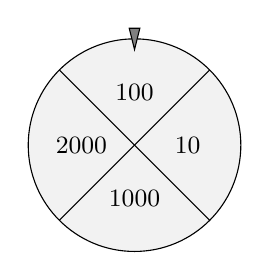
\begin{tikzpicture}[scale=1.35,font=\small] % Package pgf-pie à utiliser
\draw[fill=black!5] (0,0) circle (1);
\draw[fill=gray] (0,0.9) -- (0.05,1.1) -- (-0.05,1.1) -- cycle;
\clip (0,0) circle (1);
\draw (-2,2) -- (2,-2);
\draw (-2,-2) -- (2,2);
\node at (0.5,0) {10\euro{}};
\node at (0,0.5) {100 \euro{}};
\node at (-0.5,0) {2000\euro{}};
\node at (0,-0.5) {1000\euro{}};
\end{tikzpicture}
}
\end{exercice}

\begin{exercice}
Dans sa garde-robe, Cendrillon possède quatre robes (une noire, une rouge, une verte et une jaune), deux chapeaux (un noir et un rouge) et trois paires de chaussures (noires, rouges et vertes). Cendrillon choisit au hasard une robe, un chapeau et une paire de chaussures.

\begin{enumerate}
\item A l'aide d'un arbre, déterminer de combien de façons Cendrillon peut s'habiller.
\item Quelle est la probabilité qu'elle obtienne un ensemble d'une seule couleur ? 
\end{enumerate}
\end{exercice}

\end{multicols*}
\end{document}
